\chapter{Network in C}\label{networkC}
\section{Application layer}
We need IP protocol to use Internet. In this protocol, level 5 and 6 are hidden in Application Layer.\\
In this case, Application Layer needs to interact with Transport Layer, that is implemented in OS Kernel (Figure \ref{app_kernel}). Hence Application and Transport can talk each other with System Calls.
\begin{figure}[H]
\centering
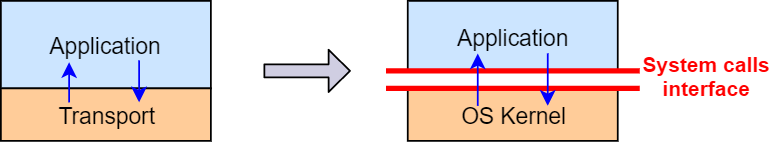
\includegraphics[scale=0.5]{Images/NetworkC/application}\caption{\footnotesize{System calls interface.}}\label{app_kernel}
\end{figure}

\section{socket()}\label{socket}
Entry-point (system call) that allow us to use the network services. It also allows application layer to access to level 4 of IP protocol. 
\begin{center}
\begin{tabular}{c}
\begin{lstlisting}[linewidth=270pt, basicstyle=\footnotesize\sffamily,]
#include <sys/types.h>
#include <sys/socket.h>

int socket(int domain, int type, int protocol);\\
\end{lstlisting}
\end{tabular}
\end{center}

\begin{table}[h]
\centering
\begin{tabular}{rcl}
\textbf{RETURN VALUE} & \multicolumn{2}{l}{\textit{File Descriptor (FD) of the socket} }\\
{} & \multicolumn{2}{l}{\textit{-1} if some error occurs and errno is set appropriately}\\
{} & \multicolumn{2}{l}{(You can check value of errno including <errno.h>).}\\
\end{tabular}
\end{table}

\begin{table}[h]
\centering
\begin{tabular}{rcl}
\textbf{domain =} & \multicolumn{2}{l}{\textit{Communication domain}}\\
{} & \multicolumn{2}{l}{protocol family which will be used for communication.}\\
{} & \textbf{AF\_INET:} & {IPv4 Internet Protocol}\\
{} & \textbf{AF\_INET6:} & {IPv6 Internet Protocol}\\
{} & \textbf{AF\_PACKET:} & {Low level packet interface}\\
& &\\
\textbf{type =} & \multicolumn{2}{l}{\textit{Communication semantics} (Figure \ref{unix_low})}\\
{} & \textbf{SOCK\_STREAM:} & {Provides sequenced, reliable, two-way, connection-based}\\
{} & {} & {bytes stream. An OUT-OF-BAND data mechanism may}\\
{} & {} & {be supported.}\\
{} & \textbf{SOCK\_DGRAM} & {Supports datagrams (connectionless, unreliable messages} \\
& & {of a fixed maximum length).}\\
& & \\
\textbf{protocol =} & \multicolumn{2}{l}{\textit{Particular protocol to be used within the socket}}\\
{} & \multicolumn{2}{l}{Normally there is only a protocol for each socket type and protocol}\\
{} & \multicolumn{2}{l}{family (protocol=0), otherwise ID of the protocol you want to use}\\
\end{tabular}
\end{table}
\begin{figure}[H]
\centering
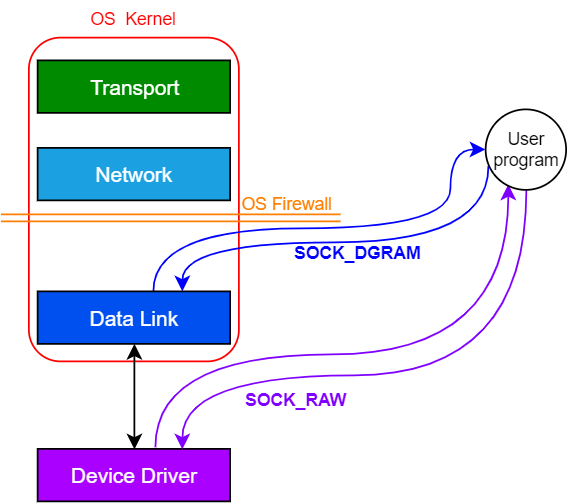
\includegraphics[scale=0.45]{Images/NetworkC/unix_low}
\caption{\footnotesize{UNIX management.}}\label{unix_low}
\end{figure}

\section{TCP connection}
In TCP connection, defined by type \textbf{SOCK\_STREAM} as written in the Section \ref{socket}, there is a client that connects to a server. It uses three primitives (related to File System primitives for management of files on disk) that do these logic actions:
\begin{enumerate}
\item{start (open bytes stream)}
\item{add/remove bytes from stream}
\item{finish (clos bytes stream)}
\end{enumerate}
TCP is used transfering big files on the network and for example with HTTP, that supports parallel download and upload (FULL-DUPLEX). The length of the stream is defined only at closure of the stream.
 
\subsection{Client}
\subsubsection{connect()}
The client calls \textbf{connect()} function, after \textbf{socket()} function of Section \ref{socket}. This function is a system call that client can use to define what is the remote terminal to which he wants to connect.

\begin{center}
\begin{tabular}{c}
\begin{lstlisting}[linewidth=370pt, basicstyle=\footnotesize\sffamily,]
#include <sys/types.h>
#include <sys/socket.h>

int connect(int sockfd, const struct sockaddr *addr,socklen_t addrlen);
\end{lstlisting}
\end{tabular}
\end{center}

\begin{table}[h]
\centering
\begin{tabular}{rcl}
\textbf{RETURN VALUE} & \multicolumn{2}{l}{\textit{0} if connection succeds}\\
{} & \multicolumn{2}{l}{\textit{-1} if some error occurs and errno is set appropriately}\\
& & \\
\textbf{sockfd =} & \multicolumn{2}{l}{\textit{Socket File Descriptor} returned by socket().}\\
& &\\
\textbf{addr =} & \multicolumn{2}{l}{\textit{Reference to struct sockaddr}}\\
{} & \multicolumn{2}{l}{sockaddr is a general structure that defines the concept of address.}\\
{} & \multicolumn{2}{l}{In practice it's a union of all the possible specific structures of each protocol.}\\
{} & \multicolumn{2}{l}{This approach is used to leave the function written in a generic way.}\\
& & \\
\textbf{addrlen =} & \multicolumn{2}{l}{\textit{Length of specific data structure used for sockaddr.}}\\
\end{tabular}
\end{table}
In the following there is the description of struct \textbf{sockaddr\_in}, that is the specific sockaddr structure implemented for family of protocls \textbf{AF\_INET}:

\begin{center}
\begin{tabular}{c}
\begin{lstlisting}[linewidth=350pt, basicstyle=\footnotesize\sffamily,]
#include <netinet/in.h>

struct sockaddr_in {
    sa_family_t    sin_family; /* address family: AF_INET */
    in_port_t      sin_port;   /* port in network byte order */
    struct in_addr sin_addr;   /* internet address */
};

/* Internet address. */
struct in_addr {
    uint32_t       s_addr;     /* address in network byte order */
};\\
\end{lstlisting}
\end{tabular}
\end{center}
The two addresses, needed to define a connection, are (see Figure \ref{addresses}):
\begin{itemize}
\item{\textbf{IP address (}$sin_addr$ in $sockaddr\_in\;\;struct$\textbf{)}\\
identifies a virtual interface in the network. It can be considered the entry-point for data arriving to the computer. \textit{It's unique in the world.}
}
\item{\textbf{Port number (}$sin_port$ in $sockaddr\_in\;\;struct$\textbf{)}\\
identifies to which application data are going to be sent. The port so must be open for that stream of data and it can be considered a service identifier. There are well known port numbers, related to standard services and others that are free to be used by the programmer for its applications (see Section \ref{files} to find which file contains well known port numbers). \textit{It's unique in the system.}
}
\end{itemize}
As mentioned in Section \ref{littleBig}, network data are organized as Big Endian, so in this case we need to insert the IP address according to this protocol. It can be done creating an array of char and analysing it as an int pointer* or with the follow function, that converts a string (E.g. "127.0.0.1") in the corresponding address:
\begin{center}
\begin{tabular}{c}
\begin{lstlisting}[linewidth=280pt, basicstyle=\footnotesize\sffamily,]
#include <sys/socket.h>
#include <netinet/in.h>
#include <arpa/inet.h>

int inet_aton(const char *cp, struct in_addr *inp);
\end{lstlisting}
\end{tabular}
\end{center}
If you want to obtain the IP address from the name of the host, using DNS, you need to use the following function that returns in h\_addr\_list the set of ip addresses related to that hostname, as arrays of characters:
\begin{center}
\begin{tabular}{c}
\begin{lstlisting}[linewidth=300pt, basicstyle=\footnotesize\sffamily,]
#include <netdb.h>
extern int h_errno;

struct hostent *gethostbyname(const char *name);

struct hostent
{
    char  *h_name;            /* official name of host */
    char **h_aliases;         /* alias list */
    int    h_addrtype;        /* host address type */
    int    h_length;          /* length of address */
    char **h_addr_list;       /* list of addresses */
}
\end{lstlisting}
\end{tabular}
\end{center}

The port number is written according to Big Endian architecture, through the next function:
\begin{center}
\begin{tabular}{c}
\begin{lstlisting}[linewidth=200pt, basicstyle=\footnotesize\sffamily,]
#include <arpa/inet.h>

uint16_t htons(uint16_t hostshort);
\end{lstlisting}
\end{tabular}
\end{center}
\begin{figure}[H]
\centering
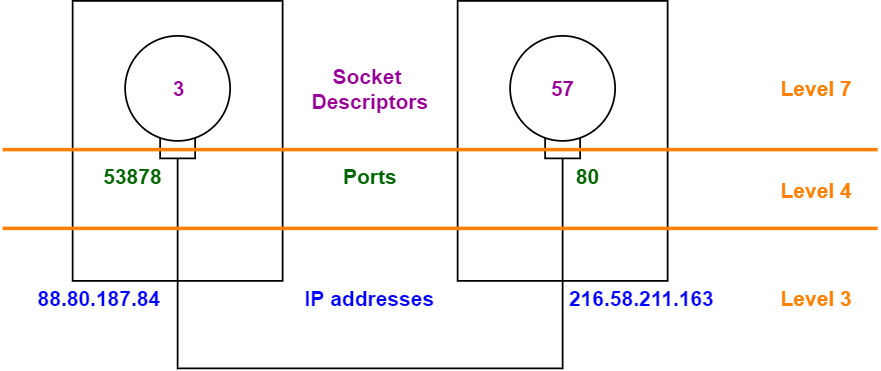
\includegraphics[scale=0.4]{Images/NetworkC/addresses}\caption{\footnotesize{After successful connection.}}\label{addresses}
\end{figure}

\subsubsection{write()}
Application protocol uses a readable string, to excange readable information (as in HTTP). This tecnique is called simple protocol and commands, sent by the protocol, are standardized and readable strings.  

\begin{center}
\begin{tabular}{c}
\begin{lstlisting}[linewidth=280pt, basicstyle=\footnotesize\sffamily,]
#include <unistd.h>

ssize_t write(int fd, const void *buf, size_t count);
\end{lstlisting}
\end{tabular}
\end{center}

\begin{table}[h]
\centering
\begin{tabular}{rcl}
\textbf{RETURN VALUE} & \multicolumn{2}{l}{\textit{Number of bytes written} on success}\\
{} & \multicolumn{2}{l}{\textit{-1} if some error occurs and errno is set appropriately}\\
& & \\
\textbf{fd =} & \multicolumn{2}{l}{\textit{Socket File Descriptor} returned by socket().}\\
& &\\
\textbf{buf =} & \multicolumn{2}{l}{\textit{Buffer of characters to write}}\\
& & \\
\textbf{count =} & \multicolumn{2}{l}{\textit{Max number of bytes to write} in the file (stream).}\\
\end{tabular}
\end{table}
The write buffer is usually a string but we don't consider the null value (\textbf{$\backslash 0$} character), that determine the end of the string, in the evaluation of count (\textbf{strlen(buf)-1}). This convention is used because \textbf{$\backslash 0$} can be part of characters stream.\\

\subsubsection{read()}
The client uses this blocking function to wait and obtain response from the remote server. Not all the request are completed immediat from the server, for the meaning of stream type of protocol. Infact in this protocol, there is a flow for which the complete sequence is defined only at the closure of it\ref{socket}.\\
\textbf{read()} is consuming bytes fom the stream asking to level 4 a portion of them, because it cannot access directly to bytes in Kernel buffer. Lower layer controls the stream of information that comes from the same layer of remove system.
\begin{center}
\begin{tabular}{c}
\begin{lstlisting}[linewidth=280pt, basicstyle=\footnotesize\sffamily,]
#include <unistd.h>

ssize_t read(int fd, void *buf, size_t count);
\end{lstlisting}
\end{tabular}
\end{center}

\begin{table}[h]
\centering
\begin{tabular}{rcl}
\textbf{RETURN VALUE} & \multicolumn{2}{l}{\textit{Number of bytes read} on success}\\
{} & \multicolumn{2}{l}{\textit{0} if EOF is reached (end of the stream)}\\
{} & \multicolumn{2}{l}{\textit{-1} if some error occurs and errno is set appropriately}\\
& & \\
\textbf{fd =} & \multicolumn{2}{l}{\textit{Socket File Descriptor} returned by socket().}\\
& &\\
\textbf{buf =} & \multicolumn{2}{l}{\textit{Buffer of characters in which it reads and stores info}}\\
& & \\
\textbf{count =} & \multicolumn{2}{l}{\textit{Max number of bytes to read} from the file (stream).}
\end{tabular}
\end{table}
So if \textbf{read()} doesn't return, this means that the stream isn't ended but the system buffer is empty.\\
If \textbf{read=0}, the function met EOF and the local system buffer is now empty. This helps client to understand that server ended before the connection.
\begin{figure}[H]
\centering
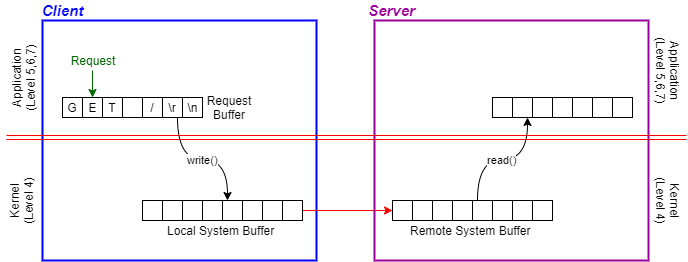
\includegraphics[scale=0.5]{Images/NetworkC/read_write1}\caption{\footnotesize{Request by the client.}}\label{rw1}
\end{figure}
\begin{figure}[H]
\centering
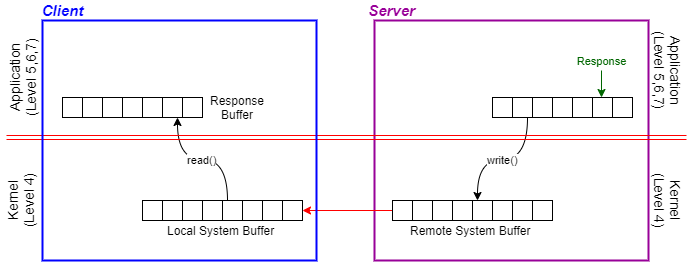
\includegraphics[scale=0.5]{Images/NetworkC/read_write2}\caption{\footnotesize{Response from the server.}}\label{rw2}
\end{figure}

\subsection{Server}
A server is a daemon, an application that works in background forever. The end of this process can be made only through the use of the Operating System.\\
The server usually uses parallel programming, to guarantee the management of more than one request simultaneously. Hence each process is composed by an infinite loop, as mentioned before.
\subsubsection{bind()}
\begin{center}
\begin{tabular}{c}
\begin{lstlisting}[linewidth=350pt, basicstyle=\footnotesize\sffamily,]
#include <sys/types.h>
#include <sys/socket.h>

int bind(int sockfd, const struct sockaddr *addr, socklen_t addrlen);
\end{lstlisting}
\end{tabular}
\end{center}

\begin{table}[h]
\centering
\begin{tabular}{rcl}
\textbf{RETURN VALUE} & \multicolumn{2}{l}{\textit{0} on success}\\
{} & \multicolumn{2}{l}{\textit{-1} if some error occurs and errno is set appropriately}\\
{} & \multicolumn{2}{l}{(You can check value of errno including <errno.h>).}\\
& & \\
\textbf{sockfd =} & \multicolumn{2}{l}{\textit{Socket File Descriptor} returned by socket().}\\
& &\\
\textbf{addr =} & \multicolumn{2}{l}{\textit{Reference to struct sockaddr}}\\
{} & \multicolumn{2}{l}{sockaddr is a general structure that defines the concept of address.}\\
& & \\
\textbf{addrlen =} & \multicolumn{2}{l}{\textit{Length of specific data structure used for sockaddr.}}\\
\end{tabular}
\end{table}

\subsubsection{listen()}
\begin{center}
\begin{tabular}{c}
\begin{lstlisting}[linewidth=185pt, basicstyle=\footnotesize\sffamily,]
#include <sys/types.h>
#include <sys/socket.h>

int listen(int sockfd, int backlog);
\end{lstlisting}
\end{tabular}
\end{center}
\begin{table}[h]
\centering
\begin{tabular}{rcl}
\textbf{RETURN VALUE} & \multicolumn{2}{l}{\textit{0} on success}\\
{} & \multicolumn{2}{l}{\textit{-1} if some error occurs and errno is set appropriately}\\
{} & \multicolumn{2}{l}{(You can check value of errno including <errno.h>).}\\
& & \\
\textbf{sockfd =} & \multicolumn{2}{l}{\textit{Socket File Descriptor} returned by socket().}\\
& &\\
\textbf{backlog =} & \multicolumn{2}{l}{\textit{Maximum length of queue of pending connections}}\\
& {The number of pending connections for sockfd can grow up}\\
& {to this value.}\\
& {The normal distribution of new requests by clients}\\
& {is usually Poisson, organized as in Figure \ref{poisson}.}
\end{tabular}
\end{table}
The listening socket, identified by \textbf{sockfd}, is unique for each association of a port number and a IP address of the server (Figure \ref{listen}).

\begin{figure}[H]
\centering
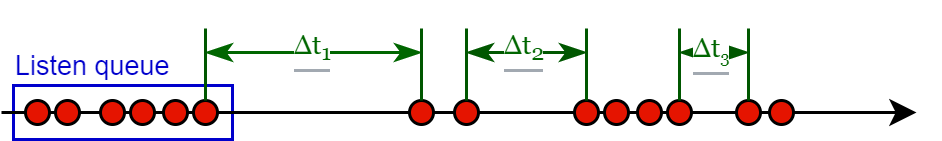
\includegraphics[scale=0.3]{Images/NetworkC/poisson}\caption{\footnotesize{Poisson distribution of connections by clients.}}\label{poisson}
\end{figure}

\begin{figure}[H]
\centering
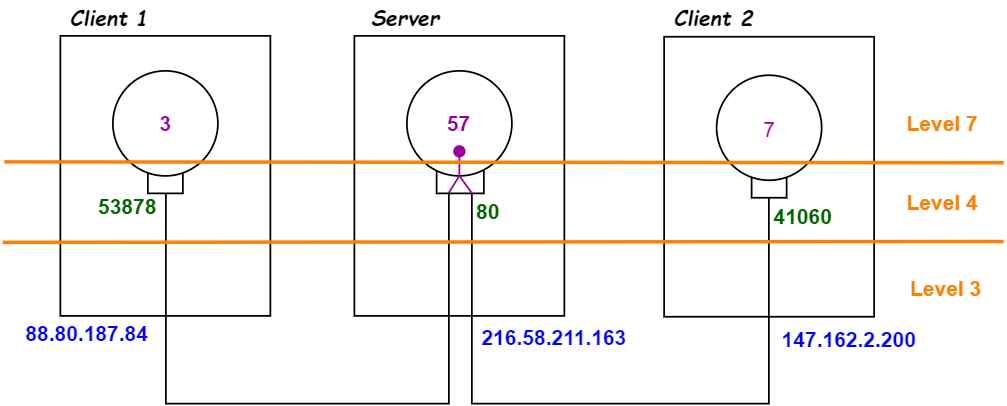
\includegraphics[scale=0.4]{Images/NetworkC/listen}\caption{\footnotesize{listen() function.}}\label{listen}
\end{figure}

\subsubsection{accept()}
\begin{center}
\begin{tabular}{c}
\begin{lstlisting}[linewidth=340pt, basicstyle=\footnotesize\sffamily,]
#include <sys/types.h>
#include <sys/socket.h>

int accept(int sockfd, struct sockaddr *addr, socklen_t *addrlen);
\end{lstlisting}
\end{tabular}
\end{center}

\begin{table}[h]
\centering\footnotesize
\begin{tabular}{rl}
\textbf{RETURN VALUE} & {\textit{Accepted Socket Descriptor}}\\
{} & {it will be used by server, to manage requests and responses from}\\
{} & {that specific client.}\\
{} & {\textit{-1} if some error occurs and errno is set appropriately}\\
{} & {(You can check value of errno including <errno.h>).}\\
& \\
\textbf{sockfd =} & {\textit{Listen Socket File Descriptor}}\\
&\\
\textbf{addr =} & {\textit{Reference to struct sockaddr}}\\
{} & {It's going to be filled by the accept() function.}\\
& \\
\textbf{addrlen =} & {\textit{Length of the struct of addr.}}\\
{} & {It's going to be filled by accept() function.}\\
{} & {( accept() is used in different cases so it can return different}\\
{} & {type of specific implementation of struct addr.)}\\
&\\
\end{tabular}
\end{table}

To manage many clients requests, we use the \textbf{accept()} function to extablish the connection one-to-one with each client, creating a uniquely socket with each client.\\
This function extracts the  first   connection request on the queue of pending connections for the listening socket \textbf{sockfd} creates a new connected socket, and returns a new file descriptor  referring  to that socket. The accept() is blocking for the server when the queue of pending requests is empty (Figure \ref{pending_accept}).\\
At lower layers of ISO/OSI, the port number and the IP Address are the same identifiers, to which listening socket is associated (Figure \ref{accept}).\\
The server needs to do a fork after doing the accept(), inside the infinite loop. Hence a new process is created to manage a new request and there is a pair client-worker for each client. So the server can be seen as it would be composed by many servers (Figure \ref{connect_accept}). 
 
\begin{figure}[H]
\centering
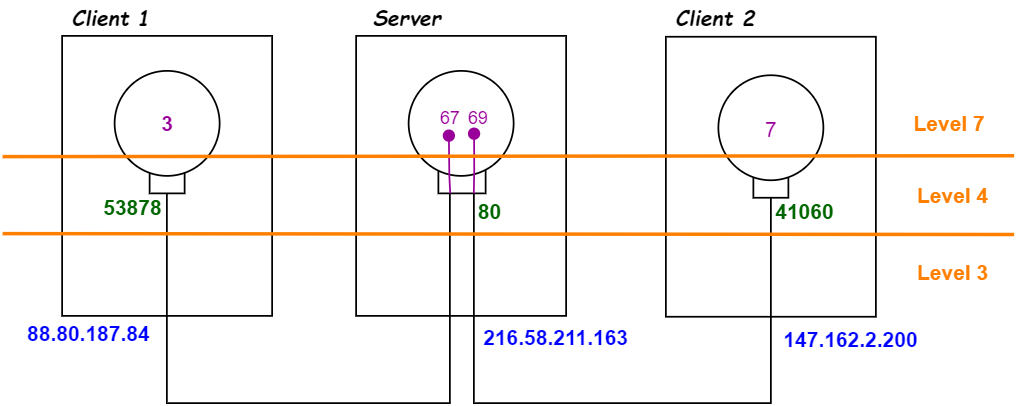
\includegraphics[scale=0.4]{Images/NetworkC/accept}\caption{\footnotesize{accept() function.}}\label{accept}
\end{figure}

\begin{figure}[H]
\centering
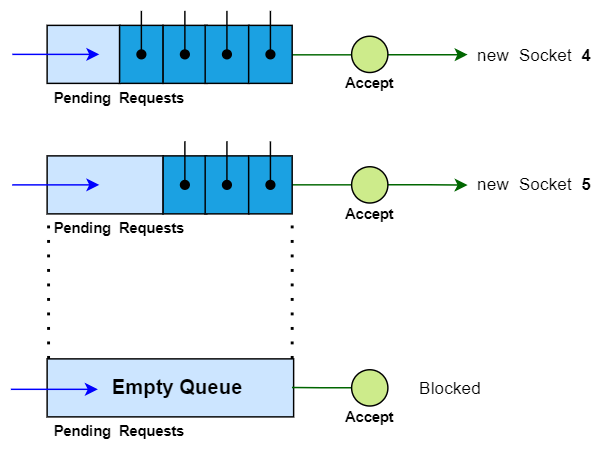
\includegraphics[scale=0.4]{Images/NetworkC/pending_accept}\caption{\footnotesize{Management of pending requests with accept().}}\label{pending_accept}
\end{figure}

\begin{figure}[H]
\centering
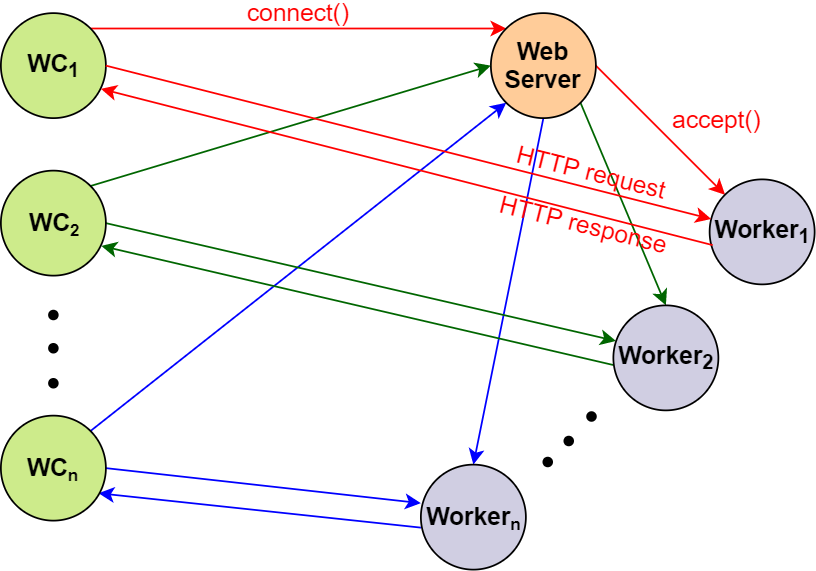
\includegraphics[scale=0.4]{Images/NetworkC/connect_accept}
\caption{\footnotesize{connect() and accept() functions in parallel server implementation.}}\label{connect_accept}
\end{figure}

\section{UDP connection}
UDP connection is defined by type \textbf{SOCK\_DGRAM} as specified in Section \ref{socket}. It's used for application in which we use small packets and we want immediate feedback directly from application. It isn't reliable because it doesn't need confirmation in transport layer.\\
It's used in Twitter application and in video streaming. \textbf{SOCK\_DGRAM} is used to read and write directly packets from/to Layer-2, with its header. Layer-2 header is added and removed by the Operating System.\\
As communication domain, as TCP connection, we can use either \textbf{AF\_INET} for IPv4 or \textbf{AF\_INET6} for IPv6. The struct sockaddr, used in this type of connection, is \textbf{struct sockaddr\_in} like in TCP because of AF\_INET domain.\\

\section{recvfrom}
This function is used to read the whole packet or frame, and only if the size of the buffer, specified as parameter, is lower than the real size of the packet, the function will split the packet and read at first the maximum size available.\\Through this function we are going to read the message packet, with format related to the packet format, depending  on which layer we are making the call.
\begin{center}
\begin{tabular}{c}
\begin{lstlisting}[linewidth=340pt, basicstyle=\footnotesize\sffamily,]
#include <sys/types.h>
#include <sys/socket.h>

ssize_t recvfrom(int sockfd, void *buf, size_t len, int flags,
                 struct sockaddr *src_addr, socklen_t *addrlen);
\end{lstlisting}
\end{tabular}
\end{center}
\begin{table}[H]
\centering\footnotesize
\begin{tabular}{rl}
\textbf{RETURN VALUE} & {\textit{Number of bytes received} on success}\\
{} & {\textit{-1} if some error occurs and errno is set appropriately}\\
{} & {(You can check value of errno including <errno.h>).}\\
& \\
\textbf{sockfd =} & {\textit{Socket File Descriptor}}\\
&\\
\textbf{buf =} & {\textit{Buffer in which the function will put the message}}\\
&\\
\textbf{len =} & {\textit{Length of the buffer buf}}\\
&{important to fullfill the buffer in input (usually buf has size}\\
&{equal to the MTU of the network).}\\
&\\
\textbf{flags =} & {\textit{Flags}}\\
{} & {added to change the behaviour of the protocol used.}\\
& \\
\textbf{src\_addr =} & {\textit{Reference to struct sockaddr}}\\
{} & {It's going to be filled by the \textbf{recvfrom()} function.}\\
& \\
\textbf{addrlen =} & {\textit{Length of the struct of addr.}}\\
{} & {It's going to be filled by accept() function.}\\
&\\
\end{tabular}
\end{table}

\section{sendto}
\begin{center}
\begin{tabular}{c}
\begin{lstlisting}[linewidth=360pt, basicstyle=\footnotesize\sffamily,]
#include <sys/types.h>
#include <sys/socket.h>

ssize_t sendto(int sockfd, const void *buf, size_t len, int flags,
               const struct sockaddr *dest_addr, socklen_t addrlen);
\end{lstlisting}
\end{tabular}
\end{center}
\begin{table}[H]
\centering\footnotesize
\begin{tabular}{rl}
\textbf{RETURN VALUE} & {\textit{Number of characters sent} on success}\\
{} & {\textit{-1} if some error occurs and errno is set appropriately}\\
{} & {(You can check value of errno including <errno.h>).}\\
& \\
\textbf{sockfd =} & {\textit{Socket File Descriptor}}\\
&\\
\textbf{buf =} & {\textit{Buffer in which the function will get the message}}\\
&\\
\textbf{len =} & {\textit{Length of the buffer buf}}\\
&{important to read the buffer in input (usually buf has size}\\
&{equal to the MTU of the network)}\\
&\\
\textbf{flags =} & {\textit{Flags}}\\
{} & {added to change the behaviour of the protocol used.}\\
& \\
\textbf{dest\_addr =} & {\textit{Reference to struct sockaddr}}\\
{} & {It's going to be filled by the \textbf{recvfrom()} function.}\\
& \\
\textbf{addrlen =} & {\textit{Length of the struct of addr.}}\\
&\\
\end{tabular}
\end{table}

\section{Lower level connection}
Creating a socket, we can also access to lower packet in ISO/OSI model, by selecting other types of communication semantics (Figure \ref{unix_low}). \textbf{SOCK\_RAW} is used to read and write directly packets from/to device driver (Layer 1), before adding Layer-2 header. The header needs to be add by us, in writing phase.\\
Using this communication semantics, we need to use the communication domain \textbf{AF\_PACKET}. The related socket is duplicated and the user program can access packets, even if it's not working at kernel level. This domain is also used to detect messages in sniffer applications (e.g. Wireshark).\\
The socket will be created through the following function call (\textit{packet(}\textbf{7}\textit{)}):
\begin{center}
\begin{tabular}{c}
\begin{lstlisting}[linewidth=340pt, basicstyle=\footnotesize\sffamily,]
int packet_socket = socket(AF_PACKET, SOCK_RAW, htons(ETH_P_ALL));
\end{lstlisting}
\end{tabular}
\end{center}
The \textbf{ETH\_P\_ALL} guarantees to receive all protocols packets.
To obtain the permission from Linux systems, we need to do the following shell command before executing the program. Otherwise the socket won't be created because the operation is not permitted.
\begin{center}
\begin{tabular}{c}
\begin{lstlisting}[linewidth=270pt, basicstyle=\footnotesize\sffamily,]
setcap cap_net_raw,cap_net_admin=eip ./my_exeutable
\end{lstlisting}
\end{tabular}
\end{center}

\subsection{Structure of Layer 2}
\begin{center}
\begin{tabular}{c}
\begin{lstlisting}[linewidth=320pt, basicstyle=\footnotesize\sffamily,]
struct sockaddr_ll {                                                                unsigned short sll_family;   /* Always AF_PACKET */                             unsigned short sll_protocol; /* Physical-layer protocol */                      int            sll_ifindex;  /* Interface number */                             unsigned short sll_hatype;   /* ARP hardware type */                            unsigned char  sll_pkttype;  /* Packet type */                                  unsigned char  sll_halen;    /* Length of address */                            unsigned char  sll_addr[8];  /* Physical-layer address */                   };
\end{lstlisting}
\end{tabular}
\end{center}
If we want to talk directly to device driver, we need to specify only two fields:
\begin{itemize}
\item{\textbf{sll\_family =} \textit{AF\_PACKET}\\
the only field common to every struct sockaddr.
}
\item{\textbf{sll\_ifindex =} \textit{index of ethernet interface}\\
to obtain it, we can call the following function:
\begin{center}
\begin{tabular}{c}
\begin{lstlisting}[linewidth=260pt, basicstyle=\footnotesize\sffamily,]
#include <net/if.h>
unsigned int if_nametoindex(const char *ifname);
\end{lstlisting}
\end{tabular}
\end{center}
\begin{table}[H]
\centering\footnotesize
\begin{tabular}{rl}
\textbf{RETURN VALUE} & {\textit{Index number of the network interface}}\\
{} & {\textit{-1} if some error occurs and errno is set appropriately}\\
{} & {(You can check value of errno including <errno.h>).}\\
& \\
\textbf{ifname =} & {\textit{Network interface name}}\\
&\\
\end{tabular}
\end{table}
Given in input the name of the network interface (e.g. \textit{"eth0"}), the function returns its related number.
}
\end{itemize}